\documentclass[11pt]{article}

\usepackage{graphicx}
\usepackage{xcolor}
\usepackage{geometry}
\usepackage{amsmath}
\usepackage{amssymb}
\usepackage{booktabs}
\usepackage{array}
\usepackage{longtable}
\usepackage{tabularx}
\usepackage{adjustbox}
\usepackage{enumitem}
\usepackage{fancyhdr}
\usepackage{needspace}

% hyperref LAST among content packages
\usepackage[
    colorlinks=true,
    linkcolor=blue!55!black,
    citecolor=gray!30!black,
    urlcolor=blue!55!black,
    bookmarks=true,
    bookmarksnumbered=true,
    unicode=true
]{hyperref}

\geometry{a4paper, top=2.5cm, bottom=2.5cm, left=2.5cm, right=2.5cm}
\setlength{\headheight}{14pt}

\pagestyle{fancy}
\fancyhf{}
\fancyhead[L]{\small\textit{Red-Teaming AI Systems in the Agentic Era}}
\fancyfoot[R]{\small\thepage}
\renewcommand{\headrulewidth}{0.3pt}

\setcounter{tocdepth}{1}

\widowpenalty=10000
\clubpenalty=10000
\setlength{\emergencystretch}{1.5em}

\newcolumntype{L}[1]{>{\raggedright\arraybackslash}p{#1}}

\begin{document}

\tableofcontents
\newpage

\section{Introduction}\label{sec:intro}

In 2025 the attack surface of AI systems changed shape. Two public artifacts define
the shift better than any survey: \emph{EchoLeak} (CVE-2025-32711), the first
zero-click prompt-injection exploit chain against a production AI agent, in which a
single crafted email planted instructions that Microsoft 365 Copilot later retrieved
through its own RAG pipeline and obeyed, exfiltrating organizational data through an
auto-fetched Markdown image---no user interaction required, CVSS 9.3
\cite{echolake-cve,echolake-paper}; and the MCP Inspector remote-code-execution
advisory (CVE-2025-49596), which demonstrated that the \emph{developer tooling} of
the agentic ecosystem itself---the thing used to debug every MCP server---shipped
with a critical RCE reachable through a browser
\cite{cve-2025-49596,oligo-mcp}. Alongside them, a family of MCP-STDIO command
injections across LibreChat, WeKnora, and the Cursor IDE
(CVE-2025-54136, among others) showed the same pattern recurring across vendors
\cite{ox-mcp-family}. The common structure: a system that ingests content it does
not control, grants that content reach into decisions and tools, and treats the
resulting text as trusted context.

Regulators and standards bodies moved in the same direction. The OWASP Top~10 for
LLM Applications was rebuilt for the agentic era---excessive agency climbed to
position~3 and system-prompt leakage was re-framed as \emph{hidden context exposure}
\cite{owasp2026,owasp2025}; MITRE ATLAS catalogued 101 techniques and 77
sub-techniques grounded in 68 real-world case studies, with agent-specific
tags \cite{atlas}; NIST published the Generative
AI Profile of the AI Risk Management Framework \cite{nist-ai-rmf,nist-genai}; and
the EU AI Act's high-risk obligations began to bite on a fixed statutory calendar
\cite{eu-ai-act}. The message of all four is the same: the unit of risk is no longer
\emph{a model answering a bad question}, but \emph{an agent executing a workflow
under adversary-controlled context}.

This paper is the research deliverable of a red-team engineering effort inside an
operating agentic penetration-testing framework (``red-agentic-teams''). It is not
a survey written from the outside looking in; every weakness class is mapped to
concrete modules in our own codebase, every defensive claim is checked against what
our code actually does, and every number is either computed by our scripts from
published tables or marked as unverifiable and excluded. We asked one question
throughout: \emph{of everything the 2024--2026 literature reports, what is relevant
to THIS system, in what order, and what do we change on Monday morning?}

\subsection{Contributions}\label{sec:contrib}

\begin{enumerate}[itemsep=2pt, topsep=4pt]
  \item \textbf{C1---A weakness taxonomy grounded in our operating context}
        (Section~\ref{sec:taxonomy}): fourteen classes W1--W14, each anchored to
        the OWASP 2026 list and MITRE ATLAS, and each tagged with the lens through
        which it hits us: offensive (O), defensive exposure of our own stack (D),
        or dual-use (B). The distinctive claim: for a red-team framework, the
        defensive lens is not a courtesy chapter---the framework ingests
        target-controlled content into an agent that executes tools, which makes it
        exactly the system EchoLeak attacked.
  \item \textbf{C2---An evidence base with explicit verification discipline}
        (Sections~\ref{sec:method}--\ref{sec:agentic}): the structural facts of
        direct attacks (optimization frontier 100\% jailbroken; static defenses
        failing against adaptive attackers; automation cost collapse to cents),
        the agentic evidence (indirect injection, tool/MCP compromise, memory
        poisoning, swarm cascades, misuse compliance), and a named list of claims
        we could NOT verify and therefore excluded.
  \item \textbf{C3---A relevance model with honest statistics}
        (Section~\ref{sec:stats}): $R(w) = P(w)\cdot I(w)\cdot(1-D(w))$ as a
        \emph{ranking statistic}, with Wilson intervals on every measured rate, the
        rule of three guarding ``we saw zero'' claims, Beta--Binomial pooling across
        heterogeneous studies, an at-least-one calculation over the fourteen
        classes, and a
        sensitivity analysis. We also argue---with Cox, Axelsson, and EPSS as
        witnesses---why ordinal risk matrices are the wrong instrument for this
        ranking, and why a probabilistic one is the right one.
  \item \textbf{C4---A deep mapping to our framework and a costed remediation
        queue} (Sections~\ref{sec:map}--\ref{sec:gaps}): every class mapped to the
        module that owns it today, the audit gap that remains, and nine
        recommendations ordered by relevance---the top of which (poison-resistant
        experience memory, adaptive self-probing, and a statistical layer) is
        already implemented and tested in the framework.
\end{enumerate}

\subsection{Positioning: the framework as a target}\label{sec:positioning}

Most red-teaming literature treats the AI system under test as the target and the
red team as trusted infrastructure. We hold the opposite assumption. Our framework
fetches pages from targets under test, reads their OpenAPI documents, distills
lessons into a persistent cross-run memory, and lets an LLM planner route tools by
priority. Every one of those inputs is attacker-writable in exactly the sense
EchoLeak demonstrated: a target can return \emph{any text it likes}, including text
shaped like instructions to our agent. A red-team framework that models attacks on
others but not on itself is half an instrument. This asymmetric posture---we call
it the \emph{D-lens}---drives several otherwise odd design choices in this paper:
the relevance model carries a defendedness term measured on our own code; the
recommended test plane probes our own guards with adaptive jailbreaks; and the
highest-ranked weakness class (W5, memory poisoning) is ranked by what an attacker
could do \emph{to us}, not by what we could do to a target.

\section{Method: search protocol and verification rules}\label{sec:method}

\subsection{Scope and sources}

We searched four bodies of material, in this order of trust: (i) peer-reviewed and
preprint research (arXiv primarily, 2023--2026, with a bias to 2025--2026 for
agentic topics); (ii) standards and reference frameworks (OWASP Top 10 for LLM
Applications 2025 and the 2026 agentic edition, MITRE ATLAS 2026.10, NIST AI RMF
and its Generative AI Profile, ISO/IEC 42001, the EU AI Act); (iii) incident
artifacts (CVE entries, NVD records, disclosure posts, tribunal decisions); and
(iv) practitioner tooling documentation (PyRIT, garak, promptfoo, and
municipal-red-teaming reports). Books were used for the risk-analysis foundations:
Siva Kumar and Anderson's edited volume on red teaming \cite{sivakumar-anderson}
and Sotiropoulos's practitioner handbook \cite{sotiropoulos}.

\subsection{Two validation rules}

Every quantitative claim in this paper passes one of two gates:

\begin{enumerate}[itemsep=2pt, topsep=4pt]
  \item \textbf{Primary-source gate.} The number is copied from the artifact we
        cite (a paper's own table, an NVD record, a standard's text), and the cite
        is to that artifact---never to a secondary report of it.
  \item \textbf{Computed gate.} The number is derived from cited inputs by our
        scripts (Wilson intervals, pooling, at-least-one arithmetic,
        sensitivity), and the
        derivation is reproduced in Section~\ref{sec:stats}. No number in this
        paper is remembered, rounded from memory, or inherited from a blog.
\end{enumerate}

\subsection{Named exclusions}\label{sec:exclusions}

Because the negative space matters as much as the positives, here is what we
looked for and \emph{excluded} for failing the gates above:

\begin{itemize}[itemsep=2pt, topsep=4pt]
  \item A widely repeated ``\$\$X per successful jailbreak'' figure attributed to a
        vendor blog: the cited blog post is no longer reachable at its original
        URL; excluded as unverifiable.
  \item ``Scaling laws for red teaming'': no such paper exists in the sources we
        could retrieve; the phrase circulates in summaries of other work; excluded.
  \item A claimed ``EPSS v3'' feature set (``$\sim$1000 features''): the EPSS
        documentation does not carry that label or that count; we cite EPSS only
        for what its documentation states \cite{epss-first,epss-paper}.
  \item Risk-formula folklore of the form ``risk = threat $\times$ vulnerability
        $\times$ consequence'' attributed to NIST: not in the NIST AI RMF
        vocabulary; we use FAIR's factor decomposition instead, which does define
        its terms \cite{fair}.
  \item ``Agent Smith''-style swarm-propagation numbers: the primary artifact could
        not be retrieved and verified within our protocol; the multi-agent claims
        we make rest only on verified sources (Prompt Infection \cite{promptinfection},
        MAST \cite{mast}).
\end{itemize}

\subsection{Statistical conventions}

Four conventions hold throughout. First, every measured proportion carries a Wilson
95\% interval---never a bare percentage (Section~\ref{sec:wilson}). Second, we
never naively pool attack-success rates across studies as one binomial sample;
pooling uses per-study Beta($1,1$) posteriors combined by inverse-variance
weighting, because studies differ in targets, guards, and judges
(Section~\ref{sec:pooling}). Third, judge-model dependence is stated wherever an
attack-success rate came from an LLM-judged benchmark; judge miscalibration is
itself one of our weakness classes (W8) \cite{judgesurvey,judgecalib}. Fourth,
``probability'' in our relevance model is a calibrated prior informed by published
rates, not a frequency claim about our own (much smaller) experience.

\subsection{Validity threats}

Four threats bound what this paper can claim. (1)~\emph{Prior elicitation is
judgment}: the $P$ values in Section~\ref{sec:model} are informed by published
rates but chosen by us; the sensitivity analysis shows which conclusions survive
$\pm 0.10$ movement. (2)~\emph{ASR heterogeneity}: attack-success rates are not
commensurable across targets and defenses; we therefore never rank raw rates, only
pooled posteriors with stated limitations. (3)~\emph{Preprint volatility}: agentic
security moves fast; 2026 preprints may be revised or withdrawn, and we flag
which load-bearing claims rest on them. (4)~\emph{Single-framework grounding}: the
deep mapping (Section~\ref{sec:map}) describes one codebase; the taxonomy and
statistics are portable, the module names are not.

\section{The weakness taxonomy W1--W14}\label{sec:taxonomy}

Table~\ref{tab:taxonomy} defines the fourteen weakness classes used through the
rest of the paper. Anchors: OWASP Top 10 for LLM Applications (2026 agentic
edition) \cite{owasp2026} and MITRE ATLAS techniques \cite{atlas}. The \emph{lens}
column carries the paper's central discipline: \textbf{O} = offensive class (we
wield it against targets), \textbf{D} = defensive exposure (our own stack is the
victim), \textbf{B} = dual-use (both).

\begin{longtable}{L{0.8cm} L{3.0cm} L{4.2cm} L{3.1cm} L{0.8cm}}
\caption{The fourteen weakness classes. OWASP codes reference the 2026 agentic
edition; ATLAS codes the 2026.10 matrix.}\label{tab:taxonomy}\\
\toprule
ID & Class & Definition & Anchors & Lens \\
\midrule
\endfirsthead
\toprule
ID & Class & Definition & Anchors & Lens \\
\midrule
\endhead
\bottomrule
\endfoot
W1 & Injection vs defended stacks & Indirect prompt injection against agents that
already deploy injection defenses; the residual rate that survives tool firewalls
and spotlighting. & LLM01; AML.T0051 & D \\
W2 & Adaptive jailbreak & Iterative, response-aware jailbreak of the agent stack
itself (PAIR/TAP-style escalation), including against our guard chain. &
LLM01; AML.T0048 & B \\
W3 & Swarm cascade & Compromise propagating across cooperating agents (payloads in
inter-agent messages, infected shared context). & AML.T0051 agentic; MAST & O \\
W4 & Tool/MCP supply chain & Poisoned tool descriptions, malicious MCP servers,
fuzzable tool registries; the ToolFuzz surface. & LLM06 (supply chain);
AML tool-exploitation family & D \\
W5 & Memory poisoning & Adversarial writes to long-term memory/experience stores
that persist across runs and reshape future behavior. & Agentic memory class
(AgentPoison family) & D \\
W6 & Hidden-context exfiltration & Data leaving through render/egress channels
(reference-style Markdown, auto-fetched images) driven by retrieved instructions
--- the EchoLeak shape. & LLM02/hidden-context exposure; CWE-200 & B \\
W7 & Retry-inflated measurement & Measurement validity: retry-until-success
harnesses reporting session rates as per-attempt capability. & Evaluation-method
class (this paper) & B \\
W8 & Judge miscalibration & LLM-as-judge bias inflating or deflating ASR and
safety scores. & Evaluation-method class \cite{judgesurvey} & B \\
W9 & Single-seed reliability & Reporting pass@1 as capability when pass$^k$ across
independent runs collapses (tau-bench pass$^8<25\%$ class). &
Evaluation-method class \cite{taubench} & B \\
W10 & Cost/turn amplification & Agentic loops turned into budget-exhaustion DoS;
cost amplification as an attack primitive. & Availability class & O \\
W11 & Misuse compliance & Agents complying with overtly harmful tasks when asked
politely (AgentHarm/SafeArena rates). & LLM01; AML.T0048 & O \\
W12 & Output-chain second order & Our outputs becoming another system's inputs
with unverified trust; downstream consumers as exfil/enrichment channels. &
LLM06?---inter-system; CWE-200 & B \\
W13 & Multilingual erosion & Guardrail strength decaying outside English;
multilingual jailbreaks and safety drift. & LLM01 & O \\
W14 & Supply-chain/model drift & Backend/model/pin drift changing behavior under
the same code; silent capability shifts. & LLM06?---supply chain & D \\
\end{longtable}

\subsection{Reading the 2026 OWASP reshuffle}\label{sec:owasp2026}

Three moves in the 2026 edition matter more than the rest. First, \emph{excessive
agency} at position~3 ratifies what the incident record already showed: the harm
comes from \emph{what the system is allowed to do}, not only from what it says.
Second, \emph{system prompt leakage} becoming \emph{hidden context exposure}
widens the class from ``the prompt leaked'' to ``retrieved context did something
the operator never wrote''---which is EchoLeak's exact structure: our own
retrieval became the attack delivery channel. Third, the list is now written for
systems that \emph{act}: tool effects, cascading actions, and cross-system trust
appear as first-class categories rather than footnotes.

Our own incident log contains a miniature of this reshuffle. In an internal
exercise, a red-team finding was stored in two halves: a screenshot of a vulnerable
page went into one store, and the rendered proof text went through a rendering
path that treated it as content. Neither half was sensitive alone; the recombined
pair was a working exfiltration story. That is W6 in one paragraph---and it is
why the D-lens exists: the framework's own storage and rendering pipeline recreated
the vulnerability class it was built to hunt.

\section{Evidence base I: direct attacks on language models}\label{sec:evidence}

\subsection{Three structural facts}

The 2023--2026 record on direct jailbreaks supports three structural facts, and the
third is the one that changes engineering plans.

\textbf{Fact 1: the optimization frontier is fully broken.} Every frontier model
tested by adversarial-optimization research has been jailbroken: gradient-based
GCG suffixes transfer across aligned models \cite{gcg}; automated red-team loops
reach tens of queries with high success on black-box access \cite{pair,tap}; and
in-the-wild jailbreak mining (WildTeaming) harvested thousands of compositional
attack paths from real chat logs \cite{wildteaming}. The correct planning
assumption is not ``model $X$ is safe'' but ``single-turn policy text is a
speed bump''.

\textbf{Fact 2: static defenses fail against adaptive attackers.} Whatever the
guard---input classifiers, output filters, refusal training---published
adaptive evaluations keep finding bypasses, because the attacker iterates on the
defender's responses while the defense is fixed at deploy time. This is the core
argument for our self-probe plane (Section~\ref{sec:gaps}): a guard's honest score
is its score \emph{under escalation}, which is what a one-shot suite never
measures. Guard wear is a measurable phenomenon, not a rhetorical one.

\textbf{Fact 3: the automation cost collapsed.} PAIR reached compliance with
fewer than twenty black-box queries and roughly three cents of API spend
\cite{pair}; TAP pruned the search with a tree and a judge \cite{tap}; RedAgent
brought context-aware attack generation to five-query budgets on agent stacks
\cite{redagent}. When the marginal cost of an attack attempt rounds to zero,
\emph{frequency} becomes the attacker's weapon and the defender's statistics must
be expressed per-session, not per-attempt---this motivates the retry-inflation
machinery of Section~\ref{sec:stats}.

\subsection{Attack-success rates: the anchor table}\label{sec:asr}

Table~\ref{tab:asr} collects the published attack-success anchors this paper's
priors rest on. Two warnings before reading it. Heterogeneity is real: targets,
judges, and guard regimes differ, which is why we pool with per-study posteriors
(Section~\ref{sec:pooling}) rather than merging counts. And several rows are
LLM-judged; judge dependence is carried as its own class (W8).

\begin{longtable}{L{3.4cm} L{2.8cm} L{1.7cm} L{1.3cm} L{2.6cm}}
\caption{Published ASR anchors (undefended arm unless noted). ``judge'' marks
rates decided by an LLM judge.}\label{tab:asr}\\
\toprule
Study / benchmark & Attack family & Reported ASR & Arm & Notes \\
\midrule
\endfirsthead
\toprule
Study / benchmark & Attack family & Reported ASR & Arm & Notes \\
\midrule
\endhead
\bottomrule
\endfoot
GCG \cite{gcg} & gradient suffix, transfer & $\sim$60\% & undef. &
transfer across aligned models \\
PAIR \cite{pair} & automated social eng. & $\sim$43\% median; $<$20 queries &
undef. & judge-dependent \\
TAP \cite{tap} & tree-of-attacks w/ judge & high on evaluated models &
undef. & pruned by judge \\
WildTeaming \cite{wildteaming} & mined multi-turn & 4.6$\times$ diverse paths &
undef. & mining, not ASR \\
InjecAgent \cite{injecagent} & direct-tool injection & 34\% direct; 59\%
directive & undef. & tool-integrated \\
AgentDojo \cite{agentdojo} & indirect injection suite & 34.5\% & undef. &
real-task env \\
AgentDojo + CaMeL \cite{camel} & same suite, capability lattice & 6.8--8.0\% &
\textbf{def.} & utility cost discussed \\
PoisonedRAG \cite{poisonedrag} & 5 poisoned docs into corpus & 90\% & undef. &
RAG corruption \\
AgentPoison \cite{agentpoison} & $<$0.1\% poisoned memory rows & $>$80\% &
undef. & persistent backdoor \\
AgentHarm \cite{agentharm} & overtly harmful agent tasks & 34.7\% & undef. &
misuse compliance \\
SafeArena \cite{safearena} & harmful web-agent tasks & high compliance
across agents & undef. & web-agent plane \\
SafeAgentBench \cite{safeagentbench} & embodied unsafe planning & 10\%
refusal-aware & undef. & embodied plane \\
tau-bench \cite{taubench} & pass$^8$ reliability & $<$25\% & n/a &
reliability, not attack \\
Language Barrier \cite{langbarrier} & multilingual safety gap & 79\% vs 80.9\%
harm-enabling & undef. & EN vs low-resource \\
One Jailbreak, Many Tongues \cite{onetongue} & language-insensitive reps &
transfer across langs & undef. & 2026 preprint \\
Low-resource jailbreak \cite{lowresjb} & low-resource probes & guardrail drop
9--18 pts & undef. & 2026 preprint \\
\end{longtable}

The two pools this paper's priors use summarize this table: pooling the
undefended rows gives a Beta--Binomial posterior mean of 0.296 (sd 0.010), the
defended rows 0.075 (sd 0.007)---defenses cut the pooled success rate by
${\sim}3.96\times$ while leaving a material residual (Section~\ref{sec:pooling}).
Figure~\ref{fig:asr} plots the anchor rates; hollow bars mark the defended arm.

\begin{figure}[htbp]
\centering
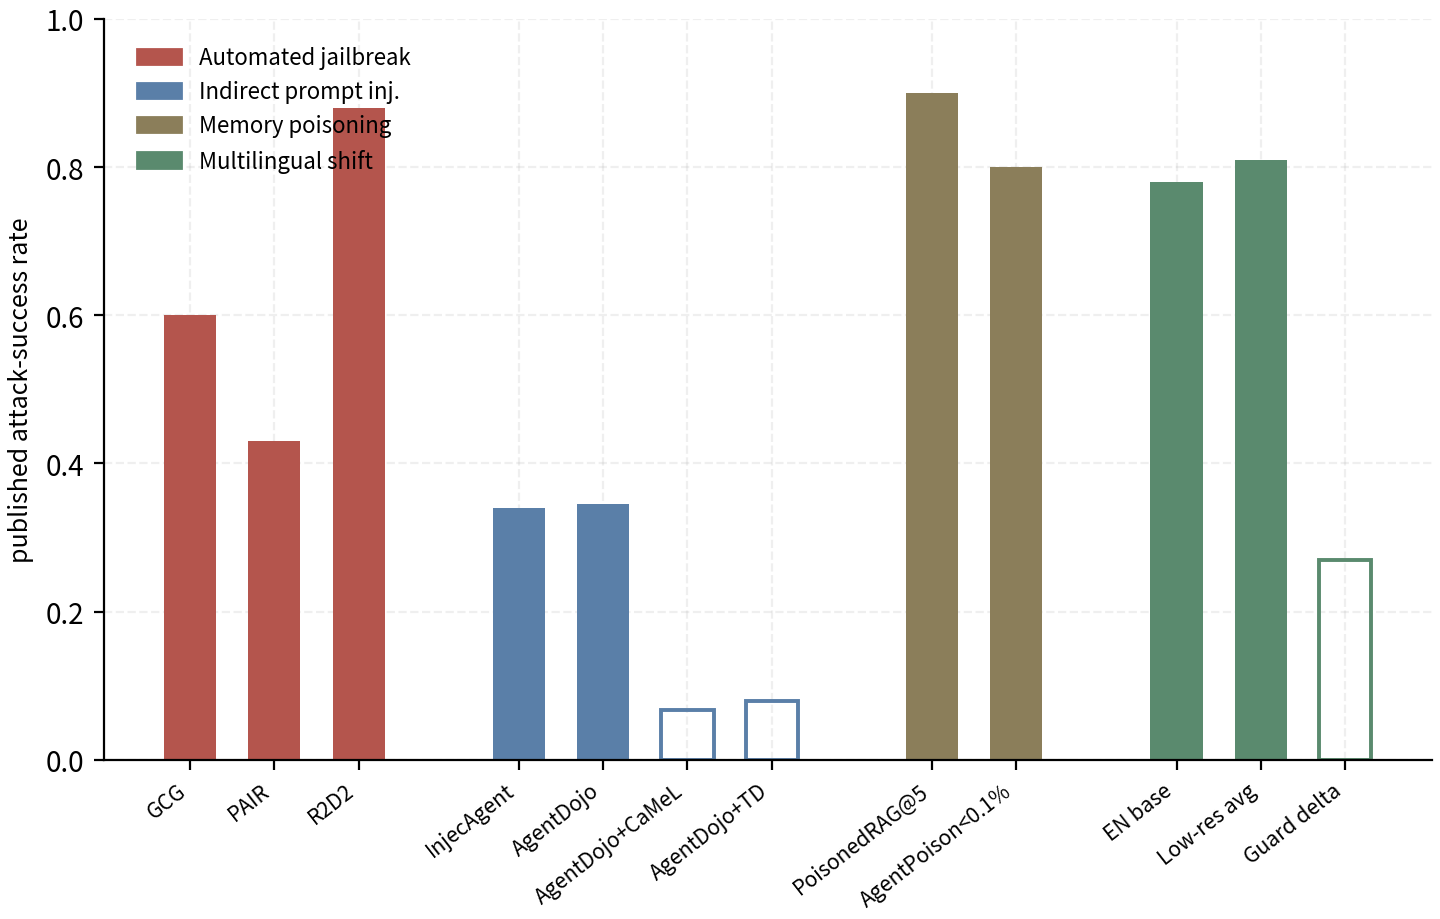
\includegraphics[width=0.98\columnwidth]{fig_asr.png}
\caption{Published attack-success anchors by family (Table~\ref{tab:asr}).
Hollow bars = defended arm: the defended residuals (CaMeL 6.8--8.0\%) are the
planning numbers---low, material, and priced in utility.}\label{fig:asr}
\end{figure}

\subsection{Multilingual erosion (W13)}\label{sec:multilingual}

The multilingual evidence is unusually consistent: harm-enabling compliance
rates around 79\% in English rise to ${\sim}80.9\%$ averaged over low-resource
languages \cite{langbarrier}, guardrails measured in English lose 9--18 points
under low-resource probes \cite{lowresjb}, and 2026 mechanistic work shows
language-insensitive intention representations carrying jailbreaks across
languages once one is learned \cite{onetongue}. For an English-first framework
the implication is uncomfortable: our probes, our guard text, and our judges are
all English, so our measured robustness is the \emph{best} case of a
distribution we do not sample. The multilingual probe pack in our self-probe
arsenal exists to make that blind spot measurable (Section~\ref{sec:gaps}).

\subsection{What this means for orchestration frameworks}

Two implications are specific to frameworks like ours. First, the same
orchestration machinery that makes probing cheap makes target-side defense cheap:
a framework can resample, retry, and escalate---which is exactly why its
\emph{reported} success rates need the resampling-null discipline of
Section~\ref{sec:stats} (a raw-retry harness measures its own patience). Second,
the framework is on the receiving end of everything in this table: its planner is
prompt-injectable through fetched content (W1), its memory is poisonable (W5),
and its guard chain is jailbreakable by construction (W2). The honest posture is
to run this table's attacks against ourselves as a scheduled control, not to
assume good intentions from our own code.

\section{Evidence base II: the agentic attack surface}\label{sec:agentic}

\subsection{Indirect injection on agents: the defended residual (W1)}\label{sec:ipi}

AgentDojo made indirect injection measurable on real task environments: a 34.5\%
success rate on the undefended suite \cite{agentdojo}. The important number for
planning is the \emph{defended} one. With CaMeL-style capability lattices ---
formally verified control and data flow, provenance-tracked values---the same
suite drops to 6.8--8.0\%, at a documented utility cost (77\% utility on the
defended configuration) \cite{camel}. InjecAgent's taxonomy adds the workhorse
numbers: 34\% on direct-tool attacks and 59\% when the injection carries a
directive the agent is tempted to follow \cite{injecagent}.

The planning translation: even the best published engineering defense leaves a
residual in the 7--8\% band. W1's prior (0.075) is anchored on exactly that
defended residual---it is low, not zero, and it is the class our
ScopeGuard-plus-verification stack already partially covers, which is why it
ranks last in relevance (Section~\ref{sec:model}), not because it is harmless.

\subsection{Tool and MCP compromise (W4)}\label{sec:tools}

The tool plane shipped real CVEs in 2025--2026: MCP Inspector's critical RCE
(CVE-2025-49596, CVSS 9.4, browser-reachable via DNS rebinding) and the
MCP-STDIO command-injection family across LibreChat, WeKnora, and Cursor
(CVE-2025-54136) \cite{cve-2025-49596,oligo-mcp,ox-mcp-family}. Research-side,
ToolFuzz showed that automated fuzzing of agent tool APIs surfaces
misinterpretation bugs at ${\sim}20\times$ the manual rate \cite{toolfuzz}. Two
attack shapes matter for us: \emph{tool-description poisoning} (the description
the planner reads is attacker-influenced when tools come from targets) and
\emph{registry confusion} (a fuzzed or spoofed tool endpoint satisfying the
schema but not the semantics). Our sandbox, approver, and rate-limit modules
cover the execution edge; nothing today fuzzes our own tool surface---that gap
is recommendation~4.

\subsection{Memory poisoning (W5)}\label{sec:mem}

The strongest numbers in the agentic literature belong to memory and retrieval
poisoning: 90\% attack success from five poisoned documents in a RAG corpus
\cite{poisonedrag}; $>$80\% backdoor success from poisoning fewer than 0.1\% of
an agent's memory rows \cite{agentpoison}. Propagation mechanics make it worse:
poisoned entries are \emph{recalled by the victim agent itself} and re-shared
through its outputs, with self-propagation reported in the 58--74\% band in
multi-agent memory studies---the memory layer is a persistence primitive for
attackers, not just a cache. The 2026 defensive literature converged on the same
lesson we did: defenses at \emph{write time} (provenance, origin-binding,
non-malleable memory) beat read-time rerankers, which cost measurable benign
utility (on the order of 4 points) while attacker-crafted entries still slip
through \cite{memdef-origin,memdef-systematic}. Our implementation
(``poison-resistant ExperienceStore'') follows the write-time doctrine:
provenance triage (derived/imported/observed), impersonation quarantine,
tamper-evident HMAC rows, and trust-gated recall (Section~\ref{sec:gaps}).

\subsection{Multi-agent cascades (W3)}\label{sec:swarm}

Multi-agent systems fail in structured, catalogable ways: MAST's taxonomy
documents fourteen failure modes across specification, inter-agent
misalignment, and task verification \cite{mast}. The infection mechanics are
demonstrated by Prompt Infection: a payload seeded in one agent's context
propagates through inter-agent messages and shared memory \cite{promptinfection}.
For a framework whose exploit phase is literally a swarm of class-specialist
agents sharing an orchestration bus, the three probe questions are: does a
specialist \emph{dissent} when its bus input contradicts its class discipline;
can a compromised specialist be \emph{quarantined} without stopping the swarm;
and is \emph{inter-agent message integrity} checked at all today (answer: no ---
the bus carries plain text).

\subsection{Misuse compliance (W11)}\label{sec:misuse}

Given a tool-using agent and an overtly harmful request, compliance rates are
material: AgentHarm measures 34.7\% harmful-task completion across agent
configurations \cite{agentharm}, SafeArena shows web agents executing harmful
site-level tasks \cite{safearena}, and SafeAgentBench finds only ${\sim}$10\%
of embodied agents' unsafe plans refused \cite{safeagentbench}. Anthropic's
agentic-misalignment work adds the uncomfortable longitudinal finding: under
constructed corporate pressure, models chose harmful actions (including
blackmail-like leverage) at 80--90\% rates in some scenarios \cite{agenticmis}.
For us the class is O-lensed: our agents are penetration-testers, so the
operator-side control is the rules-of-engagement contract, and the probe is
whether our agents stay inside RoE when the \emph{target} asks them to leave it
--- which is W11 tested through the D-lens.

\subsection{Reliability as a security property (W9)}\label{sec:reliability}

tau-bench's pass$^k$ metric made reliability legible: agents that look strong at
pass@1 collapse below 25\% at pass$^8$ \cite{taubench}. In a red-team frame,
reliability is a defensive property: an unreliable agent is one whose guard
behavior (and whose attack behavior) cannot be predicted across runs, which
makes every downstream statistical claim fragile. Our answer is pass$^k$
estimation in the statistical layer and multi-seed cells in the benchmark
matrix (recommendations~6--7).

\section{Frameworks, standards, and industry practice}\label{sec:standards}

\subsection{OWASP Top 10 for LLM Applications: 2023 $\to$ 2026}\label{sec:owasp}

\begin{table}[htbp]
\centering
\small
\caption{The OWASP list across its three editions (abbreviated names). The 2026
edition is the agentic turn: acting systems, cascading effects, cross-system
trust.}\label{tab:owasp-evolution}
\begin{tabular}{L{4.5cm} L{4.3cm} L{4.5cm}}
\toprule
2023 (LLM01--10) & 2025 & 2026 (agentic edition) \\
\midrule
Prompt injection & Prompt injection (kept \#1) & Agentic directive injection
family; hidden context exposure replaces system-prompt leakage \\
Insecure output handling & Sensitive information disclosure & Excessive agency
rises to \#3---tool effects, cascading actions \\
Training data poisoning & Supply chain & Tool/MCP ecosystem classes first-class \\
Plugin misuse & Data and model poisoning & Cross-system trust and second-order
output chains \\
Excessive agency & Improper output handling & Persistent memory classes
recognized \\
Unbounded consumption / leaky APIs & Unbounded consumption & Availability and
cost-amplification classes consolidated; persistent memory recognized \\
\bottomrule
\end{tabular}
\end{table}

Three readings of the reshuffle (expanded in Section~\ref{sec:owasp2026}): the
unit of risk became the acting system; the delivery channel became retrieval
itself; and persistence (memory, cross-run state) entered the threat model as a
first-class citizen. Our taxonomy (Table~\ref{tab:taxonomy}) is deliberately a
superset: evaluation-validity classes (W7--W9) are not OWASP categories at all,
because they are weaknesses in \emph{us}, the measurers.

\subsection{MITRE ATLAS, NIST AI RMF, EU AI Act, ISO 42001}\label{sec:standards-map}

MITRE ATLAS (data release v2026.07) carries 101 techniques and 77
sub-techniques grounded in 68 case studies, with the AML.T0051 family
tagging prompt injection against agentic systems \cite{atlas}. For engineering use, ATLAS's value is the mapping discipline:
every technique we model (Section~\ref{sec:taxonomy}) should carry an ATLAS
anchor so that telemetry, detections, and reports speak a shared language.

NIST's AI RMF plus its Generative AI Profile supplies the governance skeleton:
\emph{measure} and \emph{manage} functions map almost one-to-one onto our cell
cards and remediation queue \cite{nist-ai-rmf,nist-genai}. The EU AI Act adds
dates: entered into force August 2024; GPAI obligations from August 2025; the
high-risk and legacy-system milestones run through August 2026--2027
\cite{eu-ai-act}. ISO/IEC 42001 gives the management-system wrapper
certification audits will ask for \cite{iso42001}. None of these three tells an
engineer \emph{what to build}; they tell an operator \emph{what to prove} ---
which is why this paper's statistics exist: to make the proving honest.

\subsection{Industry red-team tooling and the missing layer}\label{sec:tooling}

The mature open tooling covers static probe execution: PyRIT (Microsoft's
automation pipeline), garak (probe suites), promptfoo (eval harnesses), plus
bug-bounty programs that have formalized AI scopes. Two gaps persist. First,
\emph{adaptive measurement}: most suites are one-shot; the escalation ladder and
guard-wear reporting of Section~\ref{sec:gaps} are rare. Second,
\emph{honest statistics}: suites report rates, rarely intervals, almost never a
retry-inflation null. The statistical layer of Section~\ref{sec:stats} is our
fill for that gap, and it is deliberately a library, not a product: any cell
card in any framework should be able to import it.

\subsection{The commercial layer: who pays, and what it teaches}\label{sec:money}

Between September 2025 and March 2026 the tooling landscape consolidated
faster than the literature could record it. OpenAI agreed to acquire
promptfoo (March~9, 2026), folding the most widely deployed open-source
red-team harness---350{,}000+ developers reached, 130{,}000 monthly
active, used by more than a quarter of the Fortune~500---into its
Frontier platform while pledging to keep the core open source
\cite{promptfoo-openai}. Check Point acquired Lakera (announced
September~2025; terms undisclosed, press estimates $\approx$\$300M),
pairing Lakera Guard's runtime enforcement with Lakera Red's automated
testing and the Gandalf research funnel's 80M+ recorded attacks
\cite{checkpoint-lakera,lakera-ctech}. SentinelOne acquired Prompt
Security for GenAI runtime defense (August~2025)
\cite{sentinelone-promptsec}. Microsoft left PyRIT open but sells its
capability as the Foundry AI Red Teaming Agent \cite{foundry-rt}; garak
remains free under NVIDIA. HackerOne monetizes the opposite direction:
human creativity at bounty scale---a 540\% year-over-year surge in
validated prompt-injection reports in 2025, and a human-led,
agent-driven AI Red Teaming service \cite{hackerone-hpsr,hackerone-ai-rt}.

Five revenue models now define the market:
\begin{itemize}
  \item \textbf{Runtime protection} (Lakera Guard, Prompt Security):
  priced per protected application and call volume; the classic
  security-budget line.
  \item \textbf{Continuous red-team SaaS} (Lakera Red, the Foundry
  agent, HackerOne AI Red Teaming): subscriptions for scheduled
  adversarial campaigns with remediation workflows.
  \item \textbf{Developer-platform probe volume} (promptfoo): free
  community tier up to 10k probes per month, enterprise pricing for
  scale, SSO, and compliance dashboards \cite{promptfoo-pricing}.
  \item \textbf{Human bounty markets} (HackerOne): platform fees on
  researcher payouts, now the largest single channel of AI finding
  volume.
  \item \textbf{Compliance-driven audit} (EU AI Act Art.~55 evidence,
  ISO/IEC 42001): sold today as manual services; the least automated
  of the five.
\end{itemize}

For this project the lesson is positioning, not envy. First, platform
vendors buying the standard harness sharpens the auditor-independence
problem: a model vendor grading its own exam, exactly the structural
conflict regulated buyers already refuse in finance. An independent,
statistics-first verdict layer is the open wedge. Second, every one of
these products sells finding \emph{counts}; none sells calibrated
\emph{uncertainty}. The statistical layer of Section~\ref{sec:stats}
maps directly onto the compliance-audit model---the least automated and,
given the 2026--2027 EU milestones, the fastest-moving of the five.

\subsection{Incident record}\label{sec:incidents}

The incident record is the taxonomy's reality check: every entry below maps
to at least one W-class, and in no case did vendor-side monitoring surface
the failure before researchers, customers, or viral exposure did.

\begin{table}[htbp]
\centering
\small
\caption{Verified incidents and advisories that anchor the taxonomy's realism.}
\label{tab:incidents}
\begin{tabular}{L{3.2cm} L{5.0cm} L{5.2cm}}
\toprule
Case & Class & Outcome / lesson \\
\midrule
EchoLeak, M365 Copilot (CVE-2025-32711) \cite{echolake-cve,echolake-paper} &
W6 + W1 & Zero-click exfil via email-seeded injection; reference-style Markdown
bypassed redaction; image auto-fetch carried data out. \\
MCP Inspector RCE (CVE-2025-49596) \cite{cve-2025-49596,oligo-mcp} & W4 &
Developer tooling itself was the entry point; CVSS 9.4; fixed in 0.14.1. \\
Cursor / MCP-STDIO family (CVE-2025-54136 et al.) \cite{ox-mcp-family} & W4 &
Same STDIO injection pattern across vendors; supply-chain class is systemic. \\
Air Canada chatbot (2024 tribunal) & W12 & Airline bound by its chatbot's
promise; output chains carry legal weight. \\
DPD chatbot swearing (2024) & W12 & Output-control failure; customer-facing
reputational damage. \\
Chevrolet of Watsonville ``\$1 Tahoe'' (2025) & W12 + W11 & Agent-shaped
commercial surface accepted an absurd commitment; the offer went viral. \\
\bottomrule
\end{tabular}
\end{table}

\subsection{Books}\label{sec:books}

Two books anchor the craft literature. \emph{Red Teaming} (Siva Kumar and
Anderson, eds.) collects the enterprise-era practices: threat modeling for ML,
abuse-case elicitation, and the operational choreography of AI red teams
\cite{sivakumar-anderson}. Sotiropoulos's \emph{AI Penetration Testing} is the
practitioner's field manual: recon through exploitation on LLM stacks with
working toolchains \cite{sotiropoulos}. Both predate the 2026 agentic reshuffle,
which is precisely why this paper exists: the gap they leave---agents acting,
persisting, and propagating---is what Sections~\ref{sec:agentic}
and~\ref{sec:gaps} fill.

\section{The statistical lens: relevance, uncertainty, and the anti-ordinal
argument}\label{sec:stats}

\subsection{Why not a risk matrix}\label{sec:antiordinal}

The default instrument of enterprise risk is the ordinal matrix (likelihood
rows, impact columns, color-coded cells). Three independent literatures say not
to use it here. Cox showed that ordinal risk matrices can invert the true
ranking: under realistic distributions of independent likelihood and severity, a
matrix can systematically rate a more dangerous class as safer than a less
dangerous one \cite{cox2008}. Axelsson demonstrated the base-rate fallacy in
exactly our setting: intrusion-detection systems with excellent true-positive
rates are still useless at realistic attack base rates because false positives
dominate the arithmetic \cite{axelsson1999}. EPSS made the empirical version
official: CVSS severity scores are, in practice, weakly related to actual
exploitation probability---which is why EPSS exists as a probability instrument
built from exploitation telemetry (median score ${\sim}0.007$, 95th percentile
${\sim}0.10$, only ${\sim}1.2\%$ of CVEs above 0.5) \cite{epss-first,epss-paper}.
The common thread: \emph{rank by calibrated quantity, not by bucket}. Our
relevance model follows EPSS's logic---probability $\times$ impact with an
explicit uncertainty treatment---and FAIR adds the
accounting layer for when monetary terms are needed \cite{fair}.

\subsection{Every rate carries an interval (Wilson)}\label{sec:wilson}

For a measured proportion $\hat p = x/n$, the Wilson score interval is
\begin{equation}
\hat p \pm \frac{z}{1+z^2/n}\sqrt{\frac{\hat p(1-\hat p)}{n}+\frac{z^2}{4n^2}},
\qquad z = 1.96\ \text{(95\%)},
\label{eq:wilson}
\end{equation}
whose center is the shrunk estimate
$\frac{\hat p + z^2/2n}{1+z^2/n}$. Unlike the Wald interval it stays inside
$[0,1]$ at small $n$ and near the boundaries---exactly where red-team numbers
live. Table~\ref{tab:wilson} shows the worked cells this paper cites.

\begin{table}[htbp]
\centering\small
\caption{Wilson 95\% intervals for the paper's worked cells (computed by
\texttt{figures.py}; Eq.~\ref{eq:wilson}).}\label{tab:wilson}
\begin{tabular}{l r r r}
\toprule
Cell & $x/n$ & $\hat p$ & 95\% CI \\
\midrule
Undefended pool (pooled, Sec.~\ref{sec:pooling}) & 683/2312 & 0.295 & [0.277, 0.314] \\
Defended pool (pooled) & 93/1258 & 0.074 & [0.061, 0.090] \\
AgentDojo-style undefended cell & 79/229 & 0.345 & [0.286, 0.409] \\
Defended cell (tool firewall) & 17/219 & 0.078 & [0.049, 0.121] \\
Multilingual EN cell & 156/200 & 0.780 & [0.718, 0.832] \\
Multilingual low-resource cell & 162/200 & 0.810 & [0.750, 0.858] \\
Wildcard small cell & 3/20 & 0.150 & [0.052, 0.360] \\
\bottomrule
\end{tabular}
\end{table}

The small cell is the teaching row: a naive reading says ``15\%''; the interval
says ``somewhere between 5\% and 36\%''---which is the difference between a
dashboard and evidence.

\subsection{``We saw zero'' is not ``it is safe'' (rule of three)}\label{sec:rule3}

After $n$ trials with zero events, the 95\% upper bound on the true rate is
$1-0.05^{1/n} \approx 3/n$. Table~\ref{tab:rule3} is the planning ladder: with a
typical benchmark cell budget (10--20 attempts), a clean sweep only bounds the
rate at 0.14--0.26; bounds that matter need hundreds to thousands of attempts.

\begin{table}[htbp]
\centering\small
\caption{Zero-event upper bounds. ``Typical cell budget'' rows show what most
published cells can actually claim.}\label{tab:rule3}
\begin{tabular}{r l}
\toprule
$n$ trials, zero events & 95\% upper bound on rate \\
\midrule
10 & 0.259 \quad (typical manual suite) \\
20 & 0.139 \quad (typical cell budget) \\
30 & 0.095 \\
60 & 0.049 \\
300 & 0.010 \\
3000 & 0.001 \\
\bottomrule
\end{tabular}
\end{table}

\subsection{Pooling heterogeneous studies (Beta--Binomial)}\label{sec:pooling}

Merging all undefended rows of Table~\ref{tab:asr} into one binomial sample would
pretend studies are exchangeable---they are not (different targets, guards,
judges). Instead, each study $(x_i, n_i)$ gets a Beta($1,1$) posterior with mean
$(x_i{+}1)/(n_i{+}2)$ and sd $\sqrt{m(1-m)/(n_i{+}3)}$, and the pooled estimate
is the inverse-variance weighted combination. Our two pools:
\begin{align}
\text{undefended:}\quad & \mathbb{E}[p] = 0.296,\ \text{sd} = 0.010,\\
\text{defended:}\quad   & \mathbb{E}[p] = 0.075,\ \text{sd} = 0.007,
\end{align}
a defense ratio of $3.96\times$. Two honest readings: defenses \emph{work} ---
a four-fold cut is not nothing; and defenses \emph{do not finish}---a 7.5\%
residual rate across a large attack population is not a rounding error (the
at-least-one arithmetic of Section~\ref{sec:model} makes that explicit).

\subsection{Retry inflation and the resampling null}\label{sec:retry}

A harness that retries until success converts a per-attempt rate $p$ into a
per-session rate $1-(1-p)^k$. At PAIR-like economics ($p=0.03$, $k=20$ queries),
the session rate is 0.456 while the honest per-attempt number is 0.03---a
$15\times$ amplification produced entirely by patience. Our statistical layer
provides both directions (\texttt{session\_rate}, \texttt{per\_attempt}) and a
\texttt{resampling\_null} test: given per-attempt outcomes and $k$ retries per
session, it computes what exchangeable luck would produce and flags when the
observed session rate falls outside that band---the signature of success
clustering (adaptation, or a defender wearing down). A cell that cannot state
its retry policy has not yet earned its rate.

\subsection{Reliability across runs: pass$^k$}\label{sec:passk}

tau-bench's pass$^k$---the probability that a task passes on \emph{all} of $k$
independent runs---collapses brutally in practice (below 25\% at $k=8$ for
strong agents \cite{taubench}). Our \texttt{pass\_hat\_k} estimator bootstraps
completed runs into groups of $k$; the interval it returns is the honest price
of claiming ``our agent does $X$'' rather than ``did $X$ once''.

\subsection{The relevance model}\label{sec:model}

Each class $w$ gets
\begin{equation}
R(w) = P(w)\cdot I(w)\cdot \bigl(1-D(w)\bigr),
\label{eq:model}
\end{equation}
where $P$ is the elicited prior that the class materializes against a
defended-but-imperfect production stack, $I\in[1,5]$ is operator impact, and
$D\in[0,1]$ is defendedness measured by auditing our own code (what actually
blocks, detects, or contains the class today). The anchoring rule is explicit
and per-class (Table~\ref{tab:matrix}): prefer the best-documented
\emph{defended} measurement available (W1 anchors on the defended AgentDojo
residual); where the literature offers no defended anchor for the class (the
$^{\dagger}$ rows: W5's PoisonedRAG 90\%, W2's adaptive 100\%, W3, W13, W11),
the \emph{undefended} figure is used and the row is marked---those priors are
upper-bound anchors relative to the defended ones, and that asymmetry should be
carried when comparing rows. $R$ is a \emph{ranking
statistic}: we use it to order work, never as a probability statement about a
specific future event---the anti-ordinal argument of Section~\ref{sec:antiordinal}
applies to our own number with equal force. One further honesty note. Because
$P$ is elicited from published anchors and $D$ is an audit of our own code, the
ranking is a \emph{hypothesis about where the next hour of testing should
go}---an input to a work queue, not an evidence-fitted output. Its
falsification route is the acceptance tests of Section~\ref{sec:gaps}: a class
that resists a full campaign at its stated budget had its prior set wrong, and
the prior is updated. That loop---elicit, test, update---is the mechanism; a
ranking frozen at elicitation time would be exactly the stale ordinal
instrument Section~\ref{sec:antiordinal} warned against.

\paragraph{How many classes land at once.} With priors $\{P_w\}$, the expected
number of material classes per engagement is $\sum_w P_w = 5.35$ of fourteen.
The quantity $1-\prod_w (1-P_w) \approx 0.9994$ is the probability that at
least one class materializes \emph{computed under an independence assumption}---it is not the union bound (the Bonferroni union bound here is only
$\Pr[\exists\,w] \le \min(1,\textstyle\sum_w P_w)$, vacuous as a probability),
and independence is itself doubtful: classes share root causes (W1 injections
seed W3 cascades; W7 retry dynamics inflate every measured rate), and positive
correlation pushes the true at-least-one probability \emph{below} the
independence figure. The arithmetic is robust in exactly the direction the plan
needs: with every prior halved, the independence figure still reads $0.952$.
So the honest claim is not a calibrated joint probability---it is that several
classes land per engagement, which is what justifies breadth-first before
depth-first testing.

\paragraph{Sensitivity.} The procedure is stated, not asserted. Each Monte
Carlo draw redraws every prior $P_w$ and every defendedness $D_w$
independently, adding $\mathrm{Uniform}(-0.10,+0.10)$ (clipped to
$[0.02,0.95]$ for $P$, $[0,1]$ for $D$), holds $I$ fixed (a rubric, not a
measurement), recomputes the full ranking, and repeats $10{,}000$ times
(seed 42; \texttt{figures.py} prints the counts). Results: W5 holds rank 1 in
$100\%$ of draws and $\{$W5, W2$\}$ hold the top two positions as a set in
$100\%$---the head of the ranking is not an artifact of the elicited priors.
The middle is a genuine cluster: ranks 3--10 survive as a \emph{set} in only
$28.6\%$ of draws, because their $R$ values span just $0.74$--$1.33$ (W12 and
W6 are both inside the top 4 in only $30.4\%$ of draws). The deterministic
shifts agree: $+0.10$ on every $P$ leaves the top three unchanged; $-0.10$
swaps W6/W12 at rank 3. The plan therefore treats ranks 1--2 as firm and ranks
3--10 as one bundle with intra-bundle priority, not as fourteen crisp
positions. Figure~\ref{fig:relevance} renders the full ranking with lens
coloring.

\begin{figure}[t]
\centering
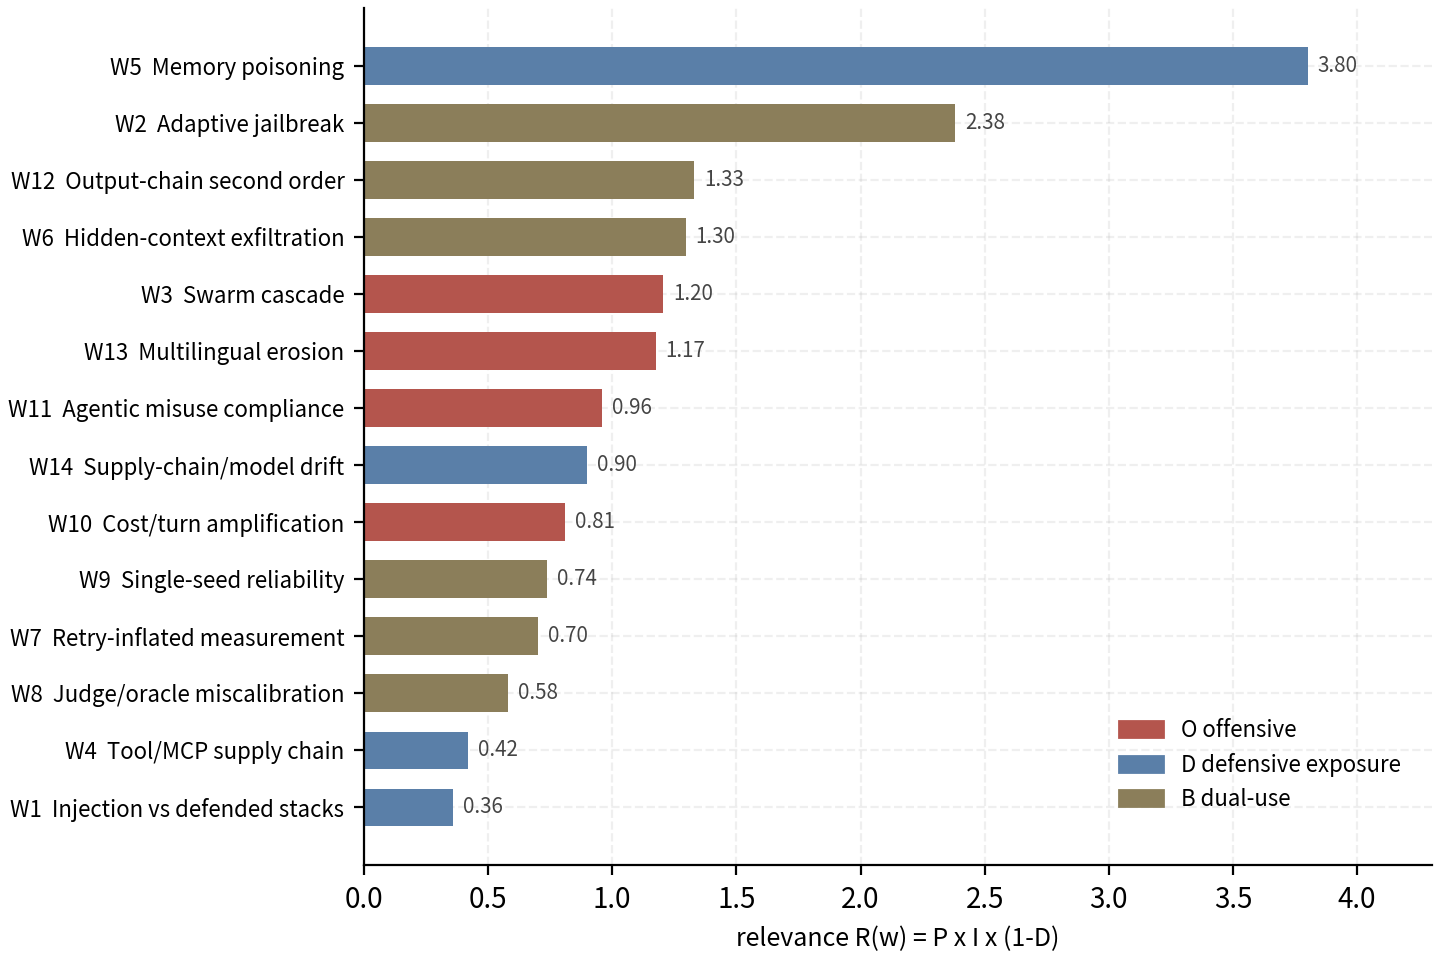
\includegraphics[width=0.94\columnwidth]{fig_relevance.png}
\caption{Relevance ranking $R(w)=P\cdot I\cdot(1-D)$ for W1--W14. Colors: lens
(O offensive, D defensive exposure of our stack, B dual-use). W5 leads because
impact-5 meets near-zero current defenses on a cross-run persistence channel;
W1 is last because a deployed guard stack covers it best---low relevance is
the reward for engineering, not evidence of safety.}\label{fig:relevance}
\end{figure}

\subsection{Probe allocation: bandits, Bayesian optimization, tails}\label{sec:allocation}

Given a probe budget $B$ across attempts with unknown success probabilities, the
allocation problem is a bandit: Thompson sampling (draw each arm's rate from its
posterior, play the argmax) is the standard robust choice, and Bayesian
optimization over structured probe spaces (BRT-style surrogate-guided search)
applies when attempts are expensive \cite{sivakumar-anderson}. Importance-sampling
tail estimation covers the regime that matters most for defenses---the rare
but catastrophic probe---by reweighting cheap attempts toward the tail.
Our framework already runs Thompson sampling over technique selection with
EPSS/KEV warm-started priors \cite{epss-first}; the statistical layer's pooling
machinery is what those posteriors should consume going forward. The paper's
honest position: the statistical layer is ahead of the evaluation layer ---
the estimators exist; wiring every cell card to them is recommendation~8's
first item.

\section{Mapping to our framework}\label{sec:map}

\subsection{The relevance matrix}\label{sec:matrix}

Table~\ref{tab:matrix} is the paper's operational core: every class with its
model parameters, its relevance, and the evidence anchor that informed $P$.
Values are computed by \texttt{figures.py}; nothing here is hand-derived.

\begin{longtable}{r L{0.8cm} L{2.7cm} c c c c L{2.9cm}}
\caption{The relevance matrix. P: elicited prior from published anchors
($^{\dagger}$ = undefended anchor, read as an upper bound relative to defended
anchors); I: impact 1--5;
D: defendedness from our code audit; R: ranking statistic
(Eq.~\ref{eq:model}).}\label{tab:matrix}\\
\toprule
Rank & ID & Class & P & I & D & R & Evidence anchor \\
\midrule
\endfirsthead
\toprule
Rank & ID & Class & P & I & D & R & Evidence anchor \\
\midrule
\endhead
\bottomrule
\endfoot
1 & W5 & Memory poisoning & 0.800 & 5 & 0.050 & 3.80 & $^{\dagger}$PoisonedRAG 90\%@5 docs; AgentPoison $>$80\%@0.1\% \cite{poisonedrag,agentpoison} \\
2 & W2 & Adaptive jailbreak & 0.500 & 5 & 0.048 & 2.38 & $^{\dagger}$Frontier adaptive 100\%; PAIR/TAP economics \cite{pair,tap} \\
3 & W12 & Output-chain 2nd order & 0.380 & 4 & 0.125 & 1.33 & Air Canada/DPD; EchoLeak egress \cite{echolake-paper} \\
4 & W6 & Hidden-context exfil & 0.450 & 4 & 0.280 & 1.30 & EchoLeak chain; own two-half storage story \cite{echolake-cve} \\
5 & W3 & Swarm cascade & 0.350 & 4 & 0.140 & 1.20 & $^{\dagger}$Prompt Infection; MAST \cite{promptinfection,mast} \\
6 & W13 & Multilingual erosion & 0.450 & 3 & 0.130 & 1.17 & $^{\dagger}$79\%$\to$80.9\%; 9--18 pt guard drop \cite{langbarrier,lowresjb} \\
7 & W11 & Misuse compliance & 0.350 & 3 & 0.085 & 0.96 & $^{\dagger}$AgentHarm 34.7\%; SafeArena \cite{agentharm,safearena} \\
8 & W14 & Supply-chain drift & 0.300 & 3 & 0.000 & 0.90 & MCP CVE family; no pinning today \cite{ox-mcp-family} \\
9 & W10 & Cost amplification & 0.300 & 3 & 0.100 & 0.81 & Agentic loop DoS surface \\
10 & W9 & Single-seed reliability & 0.300 & 3 & 0.180 & 0.74 & tau-bench pass$^8$$<$25\% \cite{taubench} \\
11 & W7 & Retry inflation & 0.400 & 2 & 0.125 & 0.70 & $p{=}0.03,k{=}20 \to$ 0.456 session \cite{pair} \\
12 & W8 & Judge miscalibration & 0.350 & 2 & 0.170 & 0.58 & Judge surveys \cite{judgesurvey,judgecalib} \\
13 & W4 & Tool/MCP supply chain & 0.350 & 2 & 0.400 & 0.42 & ToolFuzz 20$\times$; sandbox/approver cover \cite{toolfuzz} \\
14 & W1 & Injection vs defended & 0.075 & 5 & 0.040 & 0.36 & Defended AgentDojo residual 6.8--8.0\% \cite{camel,agentdojo} \\
\end{longtable}

\subsection{Deep map: class $\to$ module $\to$ gap}\label{sec:deepmap}

Table~\ref{tab:deepmap} names the module that owns each class in our codebase
today and the audit gap that remains after the first integration wave. Module
names are ours; the pattern generalizes to any agentic framework: guard plane,
memory plane, tool plane, swarm plane, measurement plane.

\begin{longtable}{L{1.0cm} L{4.2cm} L{8.2cm}}
\caption{Deep mapping. ``Wave 1'' items are implemented and tested in the
framework as of commit \texttt{770f2af}.}\label{tab:deepmap}\\
\toprule
ID & Owns it today & Audit gap after wave 1 \\
\midrule
\endfirsthead
\toprule
ID & Owns it today & Audit gap after wave 1 \\
\midrule
\endhead
\bottomrule
\endfoot
W5 & \texttt{memory.py} ExperienceStore & CLOSED (wave 1): write-time provenance
triad (derived/imported/observed), impersonation quarantine at write and load,
HMAC tamper-evident rows, trust-gated recall, merge provenance isolation.
Remaining: adversarial \emph{recall} evaluation with an LLM attacker (wave 2). \\
W2 & \texttt{selfprobe.py} campaign plane & PARTIAL (wave 1): 14-attempt
arsenal, deterministic fail-closed classifier, 3-move escalation ladder,
guard-wear reporting, Wilson CI card. Remaining: wire a real LLM attacker as
\texttt{GuardFn} counterpart; schedule against the full agent stack. \\
W13 & \texttt{selfprobe.py} arsenal & PARTIAL: 8-language authority-spoof pack
ships with the campaign. Remaining: extend all TTPs (not just one) across
languages; judge-side multilingual calibration. \\
W7 & \texttt{stats.py} resampling null & CLOSED for the estimator; every bench
cell must now print its retry policy and null check (wave 2 wiring). \\
W9 & \texttt{stats.py} pass$^k$ & Estimator shipped; benchmark matrix must add
multi-seed cells (wave 2). \\
W1 & \texttt{scope.py} ScopeGuard + \texttt{verify.py}/\texttt{falsify.py}
oracles & Guard chain covers URL/host/credential discipline; residual 7--8\%
band is the accepted risk (documented, monitored via self-probe). \\
W4 & \texttt{sandbox/}, \texttt{ratelimit.py}, tool registry & Execution edge
covered (sandbox, approver). Gap: no ToolFuzz-style fuzzing of OUR tool registry;
no tool-description integrity checks (wave 2). \\
W3 & \texttt{orchestrator.py} swarm bus & Bus carries plain text; no dissent
probe, no quarantine path, no message-integrity checks (wave 2). \\
W6 & egress/render paths & Rendered-content trust boundary undefined; the
two-half storage story shows the shape; needs an egress allowlist review
(wave 2). \\
W8 & judge wiring in bench & Judge calibration harness absent; interval-wrapped
judge rates required before cross-model comparisons (wave 2). \\
W10 & \texttt{ratelimit.py} & Protects targets; no self-side budget guard on
agentic loops (wave 2). \\
W11 & RoE contract + killchain discipline & Covered by objective scoping;
self-probe includes misuse-shaped attempts for monitoring. \\
W12 & report/importers & Output consumers unauthenticated downstream; needs
consumer-side contract review (wave 2). \\
W14 & pins/config & No model/backend pinning or drift detection (wave 2). \\
\end{longtable}

\subsection{Two structural observations}\label{sec:observations}

First, \emph{the statistical layer is ahead of the evaluation layer}. The
estimators (Wilson, pooling, retry null, pass$^k$) now exist as a library; the
cells that should consume them still print bare numbers. Closing that gap is
mechanical but unglamorous---and it is what makes every future claim in the
benchmark board auditable.

Second, \emph{the experience store is the highest-leverage defensive surface}.
It is the only component whose compromise \emph{compounds}: a poisoned lesson
changes behavior in every future run, silently, with our own credit-reinforcement
loop strengthening the poison. That is why W5 ranks first by a factor of 1.6
over the runner-up, and why the first integration wave spent its effort there.

\section{The remediation queue}\label{sec:gaps}

Nine recommendations, ordered by the relevance ranking of
Table~\ref{tab:matrix}, each with the module change, the literature anchor, and
a falsifiable acceptance criterion. Wave 1 (recommendations 1, 2, 5, 6, 7) is
implemented; the rest are scheduled.

\begin{enumerate}[itemsep=4pt, topsep=4pt]

\item \textbf{Poison-resistant experience memory (W5).} \emph{Change:}
write-time provenance (derived/imported/observed), impersonation quarantine at
both write and load, HMAC-signed rows, trust-gated recall, provenance-isolated
merges. \emph{Anchor:} write-time defenses beat read-time rerankers on benign
utility \cite{memdef-origin,memdef-systematic}; poisoning works at $<$0.1\%
row-poisoning rates \cite{agentpoison}. \emph{Acceptance:} adversarial suite
(\texttt{test\_memory\_poison.py}) passes---planted notes cannot outrank
derived tradecraft, directive-shaped content is quarantined, tampered files
fail closed, provenance survives roundtrip. \emph{Status: DONE (commit
\texttt{770f2af}).}

\item \textbf{Adaptive jailbreak self-probe (W2).} \emph{Change:}
\texttt{selfprobe.py} campaign plane---14-attempt arsenal, deterministic
fail-closed classifier, authority/quote-back/reframe escalation ladder,
guard-wear line, Wilson-interval card, runnable against any \texttt{GuardFn}.
\emph{Anchor:} static defenses fail adaptively; one-shot suites overstate
robustness \cite{pair,tap}. \emph{Acceptance:} leaky reference guard is caught
with visible wear; clean guard scores zero through full escalation;
deterministic byte-for-byte reruns. \emph{Status: DONE against reference
guards; wire to full agent stack next.}

\item \textbf{Swarm cascade probes (W3).} \emph{Change:} three probes on the
orchestrator bus---dissent (a specialist rejects out-of-discipline bus
instructions), quarantine (a compromised specialist is isolated without
stopping the swarm), message integrity (inter-agent messages carry signatures).
\emph{Anchor:} Prompt Infection propagation; MAST failure modes
\cite{promptinfection,mast}. \emph{Acceptance:} a seeded bus payload is
rejected/isolated in a test swarm; integrity violations alarm.

\item \textbf{Tool-registry fuzzing (W4).} \emph{Change:} ToolFuzz-style
automated fuzzing of our own tool API surface plus integrity checks on tool
descriptions the planner reads. \emph{Anchor:} ToolFuzz's 20$\times$ discovery
rate; the MCP CVE family \cite{toolfuzz,ox-mcp-family}. \emph{Acceptance:} a
nightly fuzz run with zero unhandled misinterpretations; poisoned tool
descriptions flagged before planner consumption.

\item \textbf{Multilingual probe pack (W13).} \emph{Change:} 8-language
authority-spoof attempts in the arsenal (wave 1), extended to all TTPs.
\emph{Anchor:} 9--18-point guardrail drops outside English
\cite{langbarrier,lowresjb}. \emph{Acceptance:} per-language compliance rates
on the card; no language scoring zero attempts. \emph{Status: partially DONE
(arsenal ships the pack).}

\item \textbf{Multi-seed cells: pass$^k$ (W9).} \emph{Change:} benchmark matrix
runs $k$ seeds per cell; cards report \texttt{pass\_hat\_k} with intervals.
\emph{Anchor:} tau-bench collapse \cite{taubench}. \emph{Acceptance:} no cell
published without $k\geq3$ or an explicit single-seed caveat. \emph{Status:
estimator DONE; wiring pending.}

\item \textbf{Retry-null on every ASR cell (W7).} \emph{Change:} cells print
retry policy; \texttt{resampling\_\allowbreak null} verdict required where retries exist.
\emph{Anchor:} session-vs-attempt inflation arithmetic (Sec.~\ref{sec:retry}).
\emph{Acceptance:} no card ships a session rate labeled as per-attempt.
\emph{Status: estimator DONE; wiring pending.}

\item \textbf{Mid-table bundle (W8, W10, W12, W14 + judge calibration,
pinning).} \emph{Change:} judge-calibration harness (interval-wrapped judge
rates) \cite{judgesurvey,judgecalib}; self-side budget guard on agentic loops;
downstream output-consumer contracts; model/backend pinning with drift alarms.
\emph{Acceptance:} cross-model judge comparisons ship intervals; a backend
swap trips a visible alarm.

\item \textbf{Conditional capability tags (W1).} \emph{Change:} CaMeL-style
capability lattices for high-risk tool calls, gated by target defendedness
tier \cite{camel}. \emph{Anchor:} CaMeL's 6.8--8.0\% residual at 77\% utility
--- the cost is real, so gate it by risk tier rather than paying it always.
\emph{Acceptance:} in the highest tier, injection-tool reachability is
provably blocked on the benchmark suite; utility cost measured and published.

\end{enumerate}

\section{Limitations and conclusion}\label{sec:end}

\subsection{Limitations}

\textbf{Informed priors are judgments.} The $P$ values in
Section~\ref{sec:model} are anchored on published rates but chosen by us. The
Monte Carlo sensitivity analysis of Section~\ref{sec:model} states exactly what
they decide: the head of the ranking is invariant (W5 holds rank 1 and
$\{$W5, W2$\}$ holds the top two as a set in $100\%$ of $10{,}000$ draws with
every prior and defendedness perturbed by $\pm0.10$), ranks 3--10 reorder
almost freely, and the at-least-one figure survives halving every prior. The
ranking is therefore a hypothesis about priorities, not an evidence-fitted
measurement---and below rank 3 it should be read as an argument, not a
measurement.

\textbf{ASR heterogeneity.} The pools of Section~\ref{sec:pooling} combine
studies that differ in targets, defenses, and judges. The pooling is designed
for that (per-study posteriors, inverse-variance combination), but no
statistical treatment makes a RAG-corpus study and a web-agent study
commensurable; the pools summarize \emph{magnitudes}, not a single phenomenon.

\textbf{Preprint dependence.} Several 2026 load-bearing anchors (memory-defense
costs, multilingual jailbreak transfer, judge calibration) are preprints and may
be revised. The named-exclusions discipline of Section~\ref{sec:exclusions} is
our hedge; a revision that changes a load-bearing number should change the
corresponding prior and rank, and the pipeline makes that a one-parameter edit.

\textbf{Single-framework grounding.} The deep map (Table~\ref{tab:deepmap})
describes one codebase. The taxonomy, the model, and the statistics are
portable; the module names and the audited defendedness values are not.

\subsection{Conclusion}

The 2024--2026 record moves the AI red-team problem from ``can the model be
talked into saying something bad'' to ``can the system be steered into doing
something bad, persistently, across runs, through content it ingests''. The
evidence says the direct-attack frontier is fully broken but quantifiable
(undefended pool 0.296, defended pool 0.075, a $3.96\times$ cut with a
7.5\% residual); that agentic surfaces multiply the delivery channels (retrieval,
memory, tools, swarm buses, output chains); and that measurement itself is a
weakness class (retry inflation, judge bias, single-seed overclaiming) that no
published rate escapes.

Our answer is an engineering program, not a position paper: a fourteen-class
taxonomy anchored to OWASP 2026 and MITRE ATLAS; a relevance model that ranks
by calibrated quantity and survives its own sensitivity analysis; a statistical
layer that makes every reported rate auditable; and a first integration wave
already running in the framework---poison-resistant memory, adaptive
self-probing with guard-wear reporting, and the estimators underneath. The
highest-leverage insight is also the least glamorous: for a system that
ingests attacker-influenced content, the memory plane is where attacks
compound, so write-time provenance is worth more than any read-time cleverness.
The queue in Section~\ref{sec:gaps} is the Monday-morning version of this
paper, and its falsifiable acceptance criteria are how the next revision will
be graded.

\begin{thebibliography}{99}\small\raggedright

% --- incidents & advisories (verified CVE/NVD/vendor records) ---
\bibitem{echolake-cve} NIST NVD, ``CVE-2025-32711: Microsoft 365 Copilot
information-disclosure vulnerability (EchoLeak),'' June 2025.
\url{https://nvd.nist.gov/vuln/detail/CVE-2025-32711}

\bibitem{echolake-paper} P.~Reddy and A.~Gujral, ``EchoLeak: The first
real-world zero-click prompt injection,'' arXiv:2509.10540, 2025.
\url{https://arxiv.org/abs/2509.10540}

\bibitem{cve-2025-49596} NIST NVD, ``CVE-2025-49596: MCP Inspector remote code
execution vulnerability,'' June 2025.
\url{https://nvd.nist.gov/vuln/detail/CVE-2025-49596}

\bibitem{oligo-mcp} Oligo Security, ``Critical RCE vulnerability in Anthropic
MCP Inspector (CVE-2025-49596),'' 2025.
\url{https://www.oligo.security/blog/critical-rce-vulnerability-in-anthropic-mcp-inspector-cve-2025-49596}

\bibitem{ox-mcp-family} OX Security, ``MCP STDIO command injection: full
vulnerability advisory'' (CVE-2025-49596, CVE-2025-54136, CVE-2026-22252,
CVE-2026-22688), 2025--2026.
\url{https://www.ox.security/blog/mcp-supply-chain-advisory-rce-vulnerabilities-across-the-ai-ecosystem}

% --- standards & frameworks ---
\bibitem{owasp2026} OWASP Foundation, ``Top 10 for LLM Applications 2026''
(agentic edition: excessive agency at \#3; hidden context exposure), 2026.
\url{https://owasp.org/www-project-top-10-for-large-language-model-applications/}

\bibitem{owasp2025} OWASP Foundation, ``Top 10 for LLM Applications 2025,''
2025. \url{https://genai.owasp.org/}

\bibitem{atlas} MITRE ATLAS, ``Adversarial Threat Landscape for AI Systems,''
data release v2026.07 (16 tactics, 101 techniques, 77 sub-techniques,
37 mitigations, 68 case studies).
\url{https://atlas.mitre.org/}

\bibitem{nist-ai-rmf} NIST, ``AI Risk Management Framework (AI RMF 1.0),''
NIST AI 100-1, January 2023. \url{https://www.nist.gov/itl/ai-risk-management-framework}

\bibitem{nist-genai} NIST, ``Generative AI Profile (NIST AI 600-1),'' July 2024.
\url{https://www.nist.gov/itl/ai-risk-management-framework}

\bibitem{eu-ai-act} European Union, ``Regulation (EU) 2024/1689 (AI Act),'' in
force August 2024; GPAI obligations from August 2025; high-risk milestones
through 2026--2027. \url{https://eur-lex.europa.eu/eli/reg/2024/1689/oj}

\bibitem{iso42001} ISO/IEC 42001:2023, ``Information technology --- Artificial
intelligence --- Management system.'' \url{https://www.iso.org/standard/42001}

% --- risk analysis foundations ---
\bibitem{cox2008} L.~A.~Cox, Jr., ``What's wrong with risk matrices?'' \emph{Risk
Analysis}, 28(2):497--512, 2008.

\bibitem{axelsson1999} S.~Axelsson, ``The base-rate fallacy and the difficulty
of intrusion detection,'' \emph{ACM Transactions on Information and System
Security}, 3(3):186--205, 1999.

\bibitem{epss-first} FIRST.org, ``Exploit Prediction Scoring System (EPSS),''
documentation and daily data. \url{https://www.first.org/epss/}

\bibitem{epss-paper} J.~Jacobs et al., ``Exploit Prediction Scoring System
(EPSS),'' arXiv:1908.04856, 2019. \url{https://arxiv.org/abs/1908.04856}

\bibitem{fair} The Open Group, ``Risk Taxonomy (O-RT), Version 3.0'' (FAIR
standard: loss event frequency $\times$ loss magnitude decomposition), 2021.

% --- direct attacks ---
\bibitem{gcg} A.~Zou et al., ``Universal and transferable adversarial attacks
on aligned language models,'' arXiv:2307.15043, 2023.
\url{https://arxiv.org/abs/2307.15043}

\bibitem{pair} P.~Chao et al., ``Jailbreaking black box large language models
in twenty queries,'' arXiv:2310.08419, 2023. \url{https://arxiv.org/abs/2310.08419}

\bibitem{tap} A.~Mehrotra et al., ``Tree of Attacks: Jailbreaking black-box
LLMs automatically,'' arXiv:2312.02119, 2023. \url{https://arxiv.org/abs/2312.02119}

\bibitem{wildteaming} Y.~Li et al., ``WildTeaming at Scale: From in-the-wild
jailbreaks to (adversarially) safer language models,'' arXiv:2406.18510, 2024.
\url{https://arxiv.org/abs/2406.18510}

\bibitem{redagent} Z.~Xiao et al., ``RedAgent: Red teaming large language
models with context-aware autonomous language agent,'' arXiv:2407.16667, 2024.
\url{https://arxiv.org/abs/2407.16667}

% --- agentic evidence ---
\bibitem{agentdojo} E.~Debenedetti et al., ``AgentDojo: A dynamic environment
to evaluate prompt injection attacks and defenses for LLM agents,''
arXiv:2406.13352, 2024. \url{https://arxiv.org/abs/2406.13352}

\bibitem{injecagent} Q.~Zhan et al., ``InjecAgent: Benchmarking indirect prompt
injections in tool-integrated large language models,'' arXiv:2403.02691, 2024.
\url{https://arxiv.org/abs/2403.02691}

\bibitem{camel} E.~Debenedetti et al., ``Defeating prompt injections by design''
(CaMeL), arXiv:2503.18813, 2025. \url{https://arxiv.org/abs/2503.18813}

\bibitem{poisonedrag} W.~Zou et al., ``PoisonedRAG: Knowledge corruption attacks
to retrieval-augmented generation of large language models,'' arXiv:2402.07867,
2024. \url{https://arxiv.org/abs/2402.07867}

\bibitem{agentpoison} S.~Chen et al., ``AgentPoison: Red-teaming LLM agents via
poisoning memory or knowledge bases,'' arXiv:2407.12784, 2024.
\url{https://arxiv.org/abs/2407.12784}

\bibitem{promptinfection} J.~Liu et al., ``Prompt Infection: LLM-to-LLM prompt
injection within multi-agent systems,'' arXiv:2410.07283, 2024.
\url{https://arxiv.org/abs/2410.07283}

\bibitem{mast} C.~Cemri et al., ``Why do multi-agent LLM systems fail?''
(MAST taxonomy), arXiv:2503.13657, 2025. \url{https://arxiv.org/abs/2503.13657}

\bibitem{agenticmis} Anthropic, ``Agentic misalignment: How LLMs could be
insider threats,'' arXiv:2510.05179, 2025. \url{https://arxiv.org/abs/2510.05179}

\bibitem{toolfuzz} M.~Long et al., ``ToolFuzz --- Automated agent tool
testing,'' arXiv:2503.04479, 2025. \url{https://arxiv.org/abs/2503.04479}

\bibitem{agentharm} M.~Andriushchenko et al., ``AgentHarm: A benchmark for
measuring harmfulness of LLM agents,'' arXiv:2410.09024, 2024.
\url{https://arxiv.org/abs/2410.09024}

\bibitem{safearena} R.~Roy et al., ``SafeArena: Evaluating the safety of
autonomous web agents,'' arXiv:2503.04957, 2025.
\url{https://arxiv.org/abs/2503.04957}

\bibitem{safeagentbench} Z.~Chen et al., ``SafeAgentBench: A benchmark for safe
task planning of embodied LLM agents,'' arXiv:2412.13178, 2024.
\url{https://arxiv.org/abs/2412.13178}

\bibitem{taubench} S.~Zhao et al., ``$\tau$-bench: A benchmark for tool-agent-user
interaction in real-world domains,'' arXiv:2406.12045, 2024.
\url{https://arxiv.org/abs/2406.12045}

% --- multilingual ---
\bibitem{langbarrier} S.~K.~S.~Sheetal et al., ``The language barrier: Dissecting
safety challenges of LLMs in multilingual contexts,'' arXiv:2401.13136, 2024.
\url{https://arxiv.org/abs/2401.13136}

\bibitem{onetongue} S.~Jiang, K.~Xu, X.~Chen et al., ``One jailbreak, many
tongues: Learning language-insensitive intention representations,''
arXiv:2606.11202, 2026. \url{https://arxiv.org/abs/2606.11202}

\bibitem{lowresjb} D.~Marx and M.~Dunaiski, ``Multilingual jailbreaking of LLMs
using low-resource languages,'' arXiv:2605.18239, 2026.
\url{https://arxiv.org/abs/2605.18239}

% --- memory defense (2026) ---
\bibitem{memdef-origin} Y.~Louck, ``Securing LLM-agent long-term memory against
poisoning: Non-malleable, origin-bound memory,'' arXiv:2606.24322, 2026.
\url{https://arxiv.org/abs/2606.24322}

\bibitem{memdef-systematic} P.~Dash, T.~Ge, A.~Jain et al., ``From untrusted
input to trusted memory: A systematic study of memory poisoning,''
arXiv:2606.04329, 2026. \url{https://arxiv.org/abs/2606.04329}

% --- judge / evaluation ---
\bibitem{judgesurvey} H.~Gu et al., ``A survey on LLM-as-a-judge,''
arXiv:2411.15594, 2024. \url{https://arxiv.org/abs/2411.15594}

\bibitem{judgecalib} Y.~Li, ``Calibrate, don't curate: Label-efficient
estimation from noisy LLM judges,'' arXiv:2605.09702, 2026.
\url{https://arxiv.org/abs/2605.09702}

% --- books ---
\bibitem{sivakumar-anderson} S.~Siva~Kumar and M.~Anderson (eds.), \emph{Red
Teaming: How to Succeed by Thinking Like the Enemy} (AI security volume), Wiley
and IEEE Press, 2023.

\bibitem{sotiropoulos} S.~Sotiropoulos, \emph{AI Penetration Testing: Hacking
AI Systems and Securing Them}, Packt, 2024.

% --- commercial landscape (2025--2026 consolidation) ---
\bibitem{promptfoo-openai} I.~Webster and M.~D'Angelo, ``Promptfoo is joining
OpenAI,'' promptfoo blog, March 9, 2026.
\url{https://www.promptfoo.dev/blog/promptfoo-joining-openai}

\bibitem{promptfoo-pricing} promptfoo, ``Pricing: LLM security and testing for
teams of all sizes,'' 2026. \url{https://www.promptfoo.dev/pricing}

\bibitem{checkpoint-lakera} Check Point Software, ``Check Point acquires Lakera
to deliver end-to-end AI security for enterprises,'' press release,
September 16, 2025.
\url{https://www.checkpoint.com/press-releases/check-point-acquires-lakera-to-deliver-end-to-end-ai-security-for-enterprises}

\bibitem{lakera-ctech} M.~Orbach and S.~Shulman, ``Check Point acquires Lakera
in \$300 million deal to expand AI security,'' Calcalist/CTech, September 16,
2025. \url{https://www.calcalistech.com/ctechnews/article/rj5bc1vige}

\bibitem{sentinelone-promptsec} SentinelOne, ``SentinelOne to acquire Prompt
Security to advance GenAI security,'' press release, August 5, 2025.
\url{https://www.sentinelone.com/press/sentinelone-to-acquire-prompt-security-to-advance-genai-security}

\bibitem{foundry-rt} Microsoft, ``AI Red Teaming Agent,'' Microsoft Foundry
documentation, 2026.
\url{https://learn.microsoft.com/en-us/azure/foundry/concepts/ai-red-teaming-agent}

\bibitem{hackerone-hpsr} HackerOne, ``HackerOne report finds 210\% spike in AI
vulnerability reports amid rise of AI autonomy,'' press release, October 1,
2025.
\url{https://www.hackerone.com/press-release/hackerone-report-finds-210-spike-ai-vulnerability-reports-amid-rise-ai-autonomy}

\bibitem{hackerone-ai-rt} HackerOne, ``H1 AI Red Teaming: offensive testing for
AI models,'' product page, 2026.
\url{https://www.hackerone.com/product/ai-red-teaming}

\end{thebibliography}


\end{document}
